\chapter[Estruturação e Implementação da Gamificação da About]{Estruturação e Implementação da Gamificação da About}

Para a implementação do trabalho, os seguintes
passos foram executados, cada um é
descrito em uma subseção: execução do teste piloto, \textit{survey} para identificação das técnicas de Gamificação,
análise estatística das técnicas, construção do \textit{framework} de Gamificação, escolha do objeto de Gamificação,
implementação das técnicas no objeto de Gamificação.
Aqui serão relatados todos os passos que foram tomados para a realização do trabalho.


% \section{Planejamento}
% \label{sec:planejamento}

% \section{Definição da Gamificação}
% \label{sec:definicao_gamification}

\section{Execução do Piloto}
\label{sec:execucao_do_piloto}
Com a intenção de validar a aplicação da About, foi implementado um piloto com as suas funcionalidades
básicas. Aqui existia apenas um post, onde o administrador um da aplicação escolhe dentre temas propostos
pelos usuários, que era postado a cada três dias.
Nesta sessão iremos descrever sobre como esta implementação foi executada.

Para desenvolver e aplicar este piloto, será necessário executar um procedimento
com os seguintes passos:

\begin{enumerate}
    \item Definir tecnologia;
    \item Desenvolver solução;
    \item Implantação em produção;
    \item Aplicar \textit{marketing} da solução para um público reduzido;
    \item Manter solução;
    \item Finalizar solução.
\end{enumerate}


Primeiramente, haviam alguns pontos necessários para a implantação da aplicação. Assim como agilidade para colocar
em produção e desenvolvimento rápido. Estes foram os padrões seguidos para a produção do piloto:


\begin{itemize}
    \item Desenvolvimento rápido;
    \item Padrões de Design simples;
    \item Escalabilidade baixa;
    \item Os usuários não carecem de executar cadastros e logins;
    \item Suporte para questionários;
    \item Facilidade de implantação.
\end{itemize}

Assim, estes pontos foram avaliados. Desta forma, era necessário implementar um software
de alta produtividade, que entregasse a funcionalidade muito rapidamente. Assim, dados estes
pontos, a tecnologia escolhida foi o WordPress, utilizando a linguagem de programação PHP.

Esta possui vários módulos prontos, desenvolvidos pela comunidade e fornecidos de maneira
gratuita. Nestes módulos, temos componentes para questionários, design de interface já
implementados facilmente e de extrema facilidade para implantação.

Como o software é considerado pequeno, não houve nenhuma necessidade de preocupação com a
infraestrutura  do sistema e com fatores técnicos ligados à alta performance. Também não foi
necessário fazer um controle de acessos e de usuários, pois a votação seria baseada no IP
do cliente, não permitindo novos acessos daquele mesmo IP.

Escolhida a tecnologia, foi iniciada a implementação da aplicação. Esta consistiu em escolher o
módulo de enquete e o módulo de layout. Após isto, tudo estava finalizado.

Para enquetes, foi
utilizado o pacote WP-Polls, este pode ser encontrado em: \url{https://wordpress.org/plugins/wp-polls/}.

Para a implementação do layout foi utilizado o módulo Amadeus, que pode ser encontrado em:
\url{https://br.wordpress.org/themes/amadeus/}.

No âmbito da implantação foi necessário apenas comprar um servidor cloud e instalar os pacotes do WordPress
dentro deste. O código fonte da aplicação pode ser encontrado neste link:
\url{https://wordpress.org/download/}.

Implementada a solução e operando, foi necessário divulgá-la para aqueles que utilizariam o código.
Então foi criado um perfil na rede social FaceBook, onde este divulgou para todos os alunos de engenharia
de software o propósito do site, bem como cada um poderia utilizá-lo. Assim, foram feitas postagens diárias
na página falando sobre as notícias da aplicação. A comunidade em si se empolgou bastante com os novos resultados.

O perfil ganhou vários seguidores que participavam ativamente ou passivamente da plataforma, respondendo, criando e
visualizando os posts realizados no projeto piloto.

Para manter a solução, era necessário levantar enquetes para o público. Então, para manter o público interessado,
foi criado uma segunda enquete que sempre estava disponível perguntando aos usuários:

Qual seria o tema que eles desejavam ver no próximo post do piloto?

Assim, todos os temas mais pedidos pelo público era lançado e operando ao longo de dois dias para uma votação.

Por fim, foi declarado que seria finalizada a solução e que o último post seria feito. Este foi realizado para a
última votação. E assim o piloto saiu de produção.

\section{Levantamento das Técnicas de Gamificação}
\label{sec:implementacao_levantamento}
Com base em uma pesquisa executada com os participantes do piloto, foi executado um levantamento das
técnicas básicas, para colocá-las frente aos objetivos estabelecidos no trabalho.

Primeiramente foi perguntado a alguns usuários que utilizaram a rede social para executar alguns
pontos relativos à impressão destes ao piloto. Detalhes sobre como estes viam as impressões passadas.
Claro que o intuito de todas as perguntas era identificar como os usuários visualizavam dinâmicas
que envolviam Gamificação dentro do piloto.

As perguntas realizadas aos usuários foram as seguintes:

\begin{quotation}
    Questão 01: Na sua opinião, o que este \textit{site} representava?
\end{quotation}

\begin{quotation}
    Questão 02: O que você acredita que motivava e levava as pessoas a utilizarem o \textit{site}?
\end{quotation}

\begin{quotation}
    Questão 03: E quanto ao contrário, o que você acredita que levava as pessoas a se desmotivarem e a não
    utilizarem mais o \textit{site}?
\end{quotation}

Assim, para estas perguntas, tivemos um total de 4 pessoas respondendo este questionário. A resposta de cada
usuário será descrita a seguir. Iremos dividir as etapas em questões. Listando assim as quatro respostas
para cada questão.


\subsection{Questão 01}
\subsubsection{Usuário 01}
A curiosidade levava as pessoas a entrarem na plataforma e descobrirem o que as
pessoas estavam falando das outras que você conhece.
\subsubsection{Usuário 02}
Era uma oportunidade de trazer a tona todos os sentimentos e sensações das pessoas
em relação as outras. Tanto relação a atitudes quanto a impressões sobre eventos
passados. Uma oportunidade de trazer visibilidade para a consequência de uma ação
feita por alguém.
\subsubsection{Usuário 03}
Criativo
\subsubsection{Usuário 04}
Um site que surgiu na faculdade, que a princípio era um portal para relatado de
acontecimentos da faculdade UnB-FGA, onde existiam vários posts inimagináveis
de algumas pessoas. E era confirmado este relato quando você via os outros comentários
anônimos, reforçando exatamente aquele ponto. Eram comentários que a princípio ninguém
acreditaria, pois eram extremamente fortes. Chegando a chocar com os fatos
declarados.

\subsection{Questão 02}
\subsubsection{Usuário 01}
As pessoas estarem curiosas para saberem sobre segredos sobre outras, que não
são contados no cotidiano.
\subsubsection{Usuário 02}
oportunidade de Conseguir punir ações erronias para as pessoas por atitudes erradas.
Mostrando que atitudes erradas tem consequência, expondo o autor caso ele faça
algo de ruim para aquele meio.
\subsubsection{Usuário 03}
curiosidade
\subsubsection{Usuário 04}
Você não queria ser um alvo do post da plataforma, você quer ser aquele que julga.
Então criava-se a curiosidade sobre os comentários feitos à minha pessoa e também
os comentários feitos a outras pessoas. O ambiente de 'fofoca' estimulava o ambiente.

\subsection{Questão 03}
\subsubsection{Usuário 01}
Medo de exposição de seus detalhes pessoas para demais indivíduos.
\subsubsection{Usuário 02}
A probabilidade de perder o controle diante da invasão de privacidade. E trazer
consequencias reais para a vida da pessoa.
\subsubsection{Usuário 03}
Falta de atualização e novidades em novos conteúdos no portal.
\subsubsection{Usuário 04}
Medo de que seu nome estivesse ali no meio da plataforma e a falta de existência
de um meio de defesa para os acusados.

Terminadas as perguntas aos usuários, foi muito claro que para todos que o que motivava
os usuários era a curiosidade, o desconhecido, a vontade de saber sobre o que
não é conhecido.

Logo, já é possível ver a presença de algumas motivações básicas de Gamificação, ligadas
à curiosidade.

Mas ainda sim, esta análise qualitativa não mostrou muito sobre quais fatores
e quais motivações básicas de fato eram percebidas no piloto executado. Assim,
como planejado, foi executado um Survey, para obter resultados quantitativos sobre
o quanto cada técnica estava influenciando o procedimento de Gamificação dentro
daquela aplicação. Estes passos serão descritos na próxima sessão.

\section{Survey das Técnicas}
\label{sec:gamifição}
Para apurar as técnicas capturadas no levantamento, foi executado um survey, a fim de dados para
embasar uma análise estatística.

Para este survey, foi utilizada uma escala de 0 a 5. Assim, foram apresentadas aos usuários
que fizeram o primeiro levantamento todas as técnicas de Gamificação, com a sua
respectiva explicação. O usuário deveria votar e dizer o quanto esta estava presente
dentro do escopo do piloto. As técnicas utilizadas são as apresentadas na sessão
\ref{sub:an_lise_estat_stica_das_t_cnicas}.

Primeiramente, para entender qual o perfil de entrevistado no trabalho, foi elaborado
um questionário prévio para traçar seus aspectos pessoais,
para que pudesse ser entendido qual a relação que esse tem com jogos e com dinâmicas
voltadas à Gamificação. Todos estes podem ser vistos neste \href{https://docs.google.com/spreadsheets/d/1galTU00NPQKaU7GRsYOciLhD0ZzIKH9BbJWyRdC3gbs/edit?usp=sharing}{link}.


Para a elaboração desta, foi apresentado um formulário a cada usuário, solicitando
que este votasse em todas as técnicas. A tabela com o resultado está neste seguinte
\href{https://docs.google.com/spreadsheets/d/1qROpsDaz32PZtkvCvmFTrqLVLgqhHR9F-Q5rcQ_pwys/edit?usp=sharing}{link}.

Assim, com esses dados obtidos, foi possível executar os cálculos da sessão \ref{sub:implementa_o_das_t_cnicas}
e montar o Framework, como apresentado no exemplo da figura \ref{fig:exoctalysis}.

Antes de executar o cálculo, foi elaborada a Tabela \ref{tab:percentual_tecnica_motivacao}
 de notas, onde é possível
observar a quantidade total possível e a quantidade de pontos feita por cada técnica.
Bem como a porcentagem que esta representa.

% Please add the following required packages to your document preamble:
% \usepackage{booktabs}
\begin{table}[]
\centering
\caption{Percentual de Técnica por Motivação Básica}
\label{tab:percentual_tecnica_motivacao}
\begin{tabular}{@{}cccc@{}}
\toprule
Motivação Básica & Pontos Totais & Pontos de Votos & Percentual \\ \midrule
1         & 68            & 140             & 48,57\%    \\
2         & 102           & 280             & 36,43\%    \\
3         & 62            & 160             & 38,75\%    \\
4         & 38            & 120             & 31,67\%    \\
5         & 93            & 200             & 46,50\%    \\
6         & 20            & 100             & 20,00\%    \\
7         & 74            & 120             & 61,67\%    \\
8         & 32            & 60              & 53,33\%    \\ \bottomrule
\end{tabular}
\end{table}

Executada esta tabela, já seria possível criar o Framework de Gamificação. Assim,
este finalizado pode ser visto na Figura.

\begin{figure}[h]
    \centering

    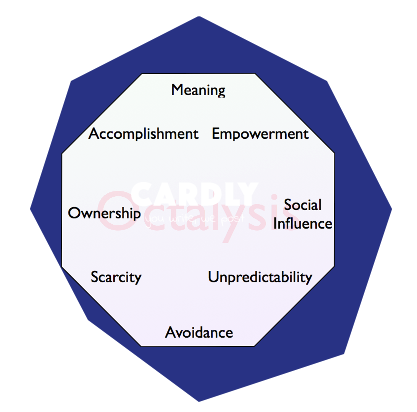
\includegraphics[width=250px, scale=1]{figuras/final_survey}
    \caption{Framework final do Survey}

    \label{fig:final_framework_octalisys}
\end{figure}

Assim, como todos estes dados, é possível iniciar um procedimento de estudo de Dados.
Todas essas análises serão feitas na próxima sessão.

\section{Análise Estatística}
\label{sec:implementacao_analise_estatistica}
Com base nestes dados, foram definidos quais as técnicas tem relação entre si para auxiliar no processo
da escolha destas para o Framework.

Todos estes estudos com base nos dados foram feitos através do resultado do survey aplicado nos usuários
da plataforma. Estes foram armazenados em uma planilha ODS.

Para fazer todas essas análises, primeiramente foi necessário escolher uma ferramenta de processamento de dados.

Como a ferramenta escolhida foi a RScript, da sessão 4.4.1, iremos proceder todos os detalhes de implementação
levando em consideração essa tecnologia.


Assim, primeiramente foi feita a instalação dos pacotes. Primeiramente é analisado
se este está instalado dentro da máquina. 
Caso esteja, o projeto vai continuar o código contrário, estes serão instalados.

\lstinputlisting[language=Python, firstline=3, lastline=10]{statistics.r}

Assim que a aplicação certifica que todos estão instalados, estes são carregados
para a aplicação da seguinte maneira:

\lstinputlisting[language=Python, firstline=12, lastline=19]{statistics.r}

Carregados todos os módulos, iniciamos em um processo de leitura da tabela ODS.
Existe uma lib na linguagem RScript para parser deste tipo de arquivo, convertendo
para dados estruturados em listas e arrays. Estes códigos podem ser vistos a seguir:

\lstinputlisting[language=Python, firstline=21, lastline=23]{statistics.r}

O algorítimo de processamento dos dados retorna um valor errado caso tenha alguma
linha de dados sem valor de votação. Assim, para resolver esses erros, foram eliminadas
todas as linhas que possuem este tipo de valor. Este processamento pode ser visto nos
comandos a seguir:

\lstinputlisting[language=Python, firstline=25, lastline=26]{statistics.r}

Agora com todos os dados tratados e prontos dentro do algorítimo, alguns cálculos podem
ser executados. Primeiramente, será criado o Alpha de Cronbach. Para isso, iremos utilizar
a lib Alpha. 

\lstinputlisting[language=Python, firstline=28, lastline=29]{statistics.r}

Dado que o Alpha foi calculado, podemos gravar em disco os três tipos de saída que são geradas.
A primeira delas é o cálculo para cada item separadamente. O segundo se trata da média destes
itens. Por fim, temos os cabeçalhos e detalhes relativos a todo o cálculo. Todos esses dados serão
salvos em disco em arquivos diferentes. 

\lstinputlisting[language=Python, firstline=31, lastline=38]{statistics.r}

Agora, será executado o resultado do algorítimo da correlação de Pearson, utilizando
também a tabela de votos sem os valores inválidos. Após, este também foi salvo em disco
com um arquivo CSV.

\lstinputlisting[language=Python, firstline=40, lastline=45]{statistics.r}

Executados todos estes passos, podemos então trabalhar com os dados executados.
Assim, foi executada uma sumarização dos dados para facilitar a visualização destes.
E são logo colocados em uma planilha CSV. Este código está disposto a seguir:

\lstinputlisting[language=Python, firstline=47, lastline=49]{statistics.r}

Para que fosse executada a aplicação do algorítimo Apriori, foi necessário fazer
algumas transformações nas operações. Entre estas estavam:

\begin{itemize}
    \item Fazer a conversão da tabela em uma matriz;
    \item Transformar valores acima de 4 em unidades binárias ligadas;
    \item Transformar valores abaixo de 4 em unidades binárias desligadas;
    \item Transformar a matriz modificada em transactions;
    \item Criar as rules utilizando o Apriori.
\end{itemize}

\lstinputlisting[language=Python, firstline=51, lastline=81]{statistics.r}

Finalizados os apuramentos de dados, foi possível analisar quais técnicas tem correlação
entre si, possibilitando assim uma orientação para a escolha de quais técnicas se interligam
e que podem vir a ser importantes para implementar na rede social About. A construção
do Framework será apresentada no próximo capítulo.

\section{Construção do Framework}
\label{sec:gamifição}
Definidas as técnicas para a implementação, estas foram utilizadas para a construção do Framework
de Gamificação.

Desta maneira, o Framework final de Gamificação foi estabelecido e pode ser visto
na figura \ref{fig:final_project_octalisys}, para executar a implementação
deste. Com a visualização dos dados analisados da sessão \ref{sec:implementacao_analise_estatistica}
e dos dados relatados pelos usuários na sessão, \ref{sec:implementacao_levantamento}, o seguinte Framework
foi construído:

\begin{figure}[h]
    \centering

    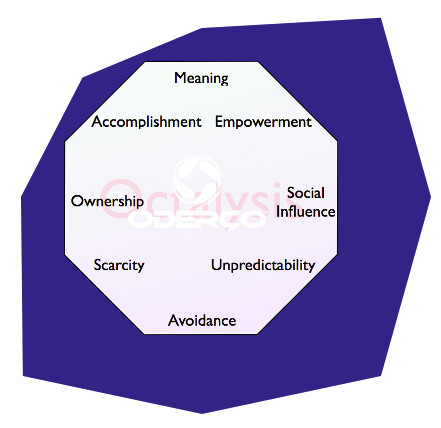
\includegraphics[width=250px, scale=1]{figuras/final_framework}
    \caption{Framework final do Projeto}

    \label{fig:final_project_octalisys}
\end{figure}

Todas estas técnicas serão aplicadas nos objetos de Gamificação que  serão definidos na próxima sessão.

\section{Objeto de Gamificação}
\label{sec:gamifição}
Assim que todo o Framework foi montado, possibilitou então que fossem escolhidos em quais
pontos da About seria possível aplicá-los. Esta sessão irá discutir sobre todos os pontos de escolha
dos objetos de Gamificação.

Como são várias técnicas de diferentes motivações básicas, esta sessão será dividida em subseções, onde
cada uma trará todas as decisões destes objetos de Gamificação. Assim, o procedimento será divido entre
as seguintes motivações: Empoderamento e Feedback, Influência Social, Imprevisibilidade,
Escassez e pra finalizar,  Perca e Rejeição.

\subsection{Objeto para Empoderamento e Feedback}
\label{sub:objeto_empoderamento_feedback}
Esta motivação básica foi implementada dentro da rede social About, para apresentar
ao usuário maneiras de que esse tivesse feedback sobre a impressão que toda a rede
tem do seu perfil. As técnicas utilizadas para tal implementação foram as seguintes:

\begin{itemize}
    \item Instant Feedback;
    \item Foice Perception.
\end{itemize}

Com essas técnicas, o usuário da base conseguirá ter de outros usuários feedbacks,
utilizando assim os abouts já escritos.

Esta motivação é importante e será aplicada nas fases de entrada e dia a dia do usuário.

\subsection{Objeto para Influência Social}
\label{sub:objeto_influencia_social}
Na rede social About, há a necessidade de que os usuários tenham relação e influência
social entre si. Este valor emocional liga os usuários e os mantém engajados para utilizar
a plataforma. Desta maneira, as seguintes técnicas foram levantadas para esta motivação
básica:

\begin{itemize}
    \item Prateleira de Troféus;
    \item Orgulho Social;
    \item Tesouro Social.
\end{itemize}

Estas técnicas foram implementadas para apresentar ao usuário diferentes meios de interação
social, bem como votar em um dado About, comentá-lo, ter troféus por abouts escritos e julgados. 
E além disso, ser apresentado aos usuários aumenta esta influência.

Esta motivação é muito importante para que o usuário se mantenha na rede social. Ela será aplicada
na fase do dia a dia do usuário.

\subsection{Objeto Imprevisibilidade \& Escassez}
\label{sub:objeto_imprevisibilidade}
Estas duas motivações básicas já estão implementadas na Rede Social About pela sua essência e foi
decidido não aplicar outras técnicas, pois estas motivações já tem técnicas suficientes implementadas.

O fato do usuário nunca saber quem irá elaborar um dado About ou quem irá votar lhe dá
todos os atributos de imprevisibilidade. Ele jamais saberá quem escreveu ou jamais terá
ideia de quem foram aqueles que votaram nestes. 

Já para quem está de fora da rede social About e vê apenas alguns abouts sendo escritos, é uma forma
de ligar a escassez com a curiosidade.

Estas duas técnicas são fundamentais para a entrada do usuário na rede social. E será implementada
nas fases de Descoberta e Entrada.

\subsection{Objeto para Perca e Rejeição}
\label{sub:objeto_perca_rejeicao}
Esta técnica foi utilizada como parte importante do projeto para motivar o usuário a não deixar a rede
social e sempre estar atualizando e participando. Para esta motivação, foi implementada a seguinte técnica:

\begin{itemize}
    \item FOMO Ponch.
\end{itemize}

Esta foi utilizada como forma do usuário perder pontos na rede social caso não escreva um About para alguém
dentro de um determinado período de tempo. Assim, a cada dia consecutivo que este está ativo
, ele ganha pontos ao escrever abouts. Caso passe um dia sem escrever, a sua pontuação volta ao início, adicionando
poucos pontos a cada About criado.

Esta motivação será aplicada na fase de fim de jogo do usuário, motivando-o a sempre entrar na plataforma
e não deixar de escrever abouts.

\section{Implementação das Técnicas}
\label{sec:gamifição}
Assim que todo o Framework foi estabelecido e seus objetos também, foi possível implementar
na rede social todos os pontos para colocar estas técnicas em prática.
